\def\linkdethi{} %Đường link cần dẫn tới
\anmaQR
%%%%%%%%%%%%%%%%%%%%%%%%
\def\toanlop{12}
\def\thoigian{90}
\def\namhoc{2025 - 2026}
\begin{dethi}
	{Bộ GD\&ĐT}
	{VTED ft KING EDU}
	{TDMT13}
	{Đề thi thử THPTQG 2026}
\end{dethi}
\caulc
\Opensolutionfile{ans}[ans/ansTN-Dung]
%%%%=============EX_1=============%%%
%\begin{ex}%[2D4N1-4]%[TDMT13]%[Mui Doan]
%	Họ nguyên hàm của hàm số $f(x) = 3^{x+1}$ là
%	\choice
%	{\True $\dfrac{3^{x+1}}{\ln 3} + C$}
%	{$\dfrac{3^x}{\ln 3} + C$}
%	{$\dfrac{3^{x+2}}{x+2} + C$}
%	{$3^{x+1} + C$}
%	\loigiai{
%		Ta có $\displaystyle\int f(x)\mathrm{\,d}x=\displaystyle\int 3^{x+1}\mathrm{\,d}x=\dfrac{3^{x+1}}{\ln 3} + C$.
%	}
%\end{ex}
%%%%=============================%%%
%
%%%%=============EX_2=============%%%
%\begin{ex}%[2D4H3-1]%[TDMT13]%[Huỳnh Trí Thiện]
%	Diện tích hình phẳng giới hạn bởi các đường $y=f(x)$, $y=g(x)$, $x=a$, $x=b$ ($a<b$) được tính theo công thức
%	\choice
%	{$S = \pi \displaystyle\int\limits_a^b \left| f(x) - g(x) \right| \mathrm{\,d}x$}
%	{\True $S = \displaystyle\int\limits_a^b \left| f(x) - g(x) \right| \mathrm{\,d}x$}
%	{$S = \displaystyle\int\limits_a^b \left[ f(x) - g(x) \right] \mathrm{\,d}x$}
%	{$S = \displaystyle\int\limits_a^b \left| f(x) \right| \mathrm{\,d}x - \displaystyle\int\limits_a^b \left| g(x) \right| \mathrm{\,d}x$}
%	\loigiai{
%		Diện tích hình phẳng giới hạn bởi đồ thị hàm số $y=f(x)$, $y=g(x)$ liên tục trên đoạn $[a;b]$ và hai đường thẳng $x=a$, $x=b$ ($a<b$) được tính bằng công thức
%		\[ S = \displaystyle\int\limits_a^b \left| f(x) - g(x) \right| \mathrm{\,d}x. \]
%	}
%\end{ex}
%%%%=============================%%%
%
%%%%=============EX_3=============%%%
%\begin{ex}%[2D3H2-2]%[TDMT13]%[Chu Hà]
%	Cho hai mẫu số liệu ghép nhóm $M_1$, $M_2$ với bảng tần số ghép nhóm như sau
%	\begin{center}
%		\begin{tabular}{|c|c|c|c|c|c|c|c|}
%			\hline
%			\multirow{2}{*}{$M_1$} & Nhóm & $[5;7)$ & $[7;9)$ & $[9;11)$ & $[11;13)$ & $[13;15)$ & $[15;17)$\\
%			\cline{2-8}
%			& Tần số & $3$ & $5$ & $6$ & $4$ & $6$ & $9$\\
%			\hline
%			\multirow{2}{*}{$M_2$} & Nhóm & $[5;7)$ & $[7;9)$ & $[9;11)$ & $[11;13)$ & $[13;15)$ & $[15;17)$\\
%			\cline{2-8}
%			& Tần số & $6$ & $10$ & $12$ & $8$ & $12$ & $18$\\
%			\hline
%		\end{tabular}
%	\end{center}
%	Hãy so sánh độ lệch chuẩn $s_1$, $s_2$ của hai mẫu số liệu $M_1$, $M_2$.
%	\choice
%	{$s_1<s_2$}
%	{\True $s_1=s_2$}
%	{$s_1=2s_2$}
%	{$s_1=3s_2$}
%	\loigiai{
%		Ta thấy tần số của $M_2$ gấp đôi tần số của $M_1$ ở mọi nhóm.\\
%		Do đó các giá trị đại diện không thay đổi, chỉ số lần xuất hiện tăng đều theo cùng một tỷ lệ.\\
%		Suy ra số trung bình và phương sai của hai mẫu là như nhau, nên độ lệch chuẩn cũng bằng nhau.\\
%		Vậy $s_1=s_2$.
%	}
%\end{ex}
%%%%=============================%%%
%
%%%%=============EX_4=============%%%
%\begin{ex}%[2D1N2-2]%[TDMT13]%[Nguyễn Tấn Linh]
%	\immini[thm]{Cho hàm số $y = ax^3 + bx^2 + cx + d$ ($a \neq 0$) có đồ thị như hình vẽ.
%		Giá trị cực đại của hàm số là
%		\choice
%		{$1$}
%		{\True $2$}
%		{$(1; 2)$}
%		{$-1$}}{
%		\begin{tikzpicture}[scale=.5,line cap=butt,line join=miter,>=stealth]
%			\draw[->] (-3,0)--(4,0)
%			node[shift={(-100:7pt)},font=\scriptsize]{$x$};
%			\draw[->] (0,-2)--(0,3)
%			node[shift={(180:7pt)},font=\scriptsize]{$y$};
%			\draw (5pt,0) |- (0,5pt)
%			(0,0) node[shift={(225:9pt)},font=\scriptsize]{$O$};
%			\foreach \x in {2}{
%				\draw (\x,1.5pt)--(\x,-1.5pt) node[font=\scriptsize,shift={(90:7pt)}]{\x};
%			}
%			\foreach \y in {2}{
%				\draw (1.5pt,\y)--(-1.5pt,\y) node[font=\scriptsize,shift={(0:7pt)}]{\y};
%			}
%			\draw[dashed] (-1,2)--(0,2)
%			(2,0)--(2,-1.85);
%			\tikzset{declare function={f (\x)=2/7*(\x)^3-3/7*(\x)^2-12/7*(\x)+1;}}
%			\foreach \x/\y in {-1/2,0/2,2/0,0/0,2/-1.85}{
%				\fill (\x,\y) circle (1pt);
%			}
%			\begin{scope}
%				\draw[samples=100] plot[domain=-2.5:3.5] (\x,{f (\x)});
%			\end{scope}
%		\end{tikzpicture}
%	}
%	\loigiai{
%		Dựa vào đồ thị, ta thấy điểm cực đại của đồ thị hàm số có tung độ bằng $2$.\\
%		Do đó, giá trị cực đại của hàm số là $y_{\text{CĐ}} = 2$.
%	}
%\end{ex}
%%%%=============================%%%
%
%%%%=============EX_5=============%%%
%\begin{ex}%[2H5N2-3]%[TDMT13]%[Phạm Hải Dương]
%	Trong không gian $Oxyz$, phương trình tham số của trục $Ox$ là
%	\choice
%	{$\heva{&x=0\\&y=t\\&z=0}$}
%	{$\heva{&x=0\\&y=t\\&z=t }$}
%	{$\heva{&x=0\\&y=0\\&z=t}$}
%	{\True $\heva{&x=t\\&y = 0\\&z = 0}$}
%	\loigiai{
%		Trục $Ox$ đi qua gốc tọa độ $O(0;0;0)$ và có vectơ chỉ phương là $\overrightarrow{i} = (1;0;0)$.\\
%		Do đó, phương trình tham số của trục $Ox$ là $\heva{&x=t\\&y=0\\&z=0}$ với $t \in \mathbb{R}$.
%	}
%\end{ex}
%%%%=============================%%%
%
%%%%=============EX_6=============%%%
%\begin{ex}%[1D6H4-3]%[TDMT13]%[Nguyễn Sơn Thành]
%	Tập nghiệm của bất phương trình $\log (x-3)<1$ là
%	\choice
%	{$\{3; 13\}$}
%	{$(-\infty; 13)$}
%	{$(13; +\infty)$}
%	{\True $(3; 13)$}
%	\loigiai{
%		Điều kiện xác định $x-3>0\Leftrightarrow x>3$.\\
%		Ta có $\log (x-3)<1\Leftrightarrow x-3<10^1\Leftrightarrow x <13$.\\
%		Kết hợp điều kiện xác định $x>3$ ta có tập nghiệm của bất phương trình là $(3; 13)$.
%	}
%\end{ex}
%%%%=============================%%%
%
%%%%=============EX_7=============%%%
%\begin{ex}%[2H5N1-2]%[TDMT13]%[Bồ Văn Hậu]
%	Trong không gian $Oxyz$, cho phương trình mặt phẳng $(\alpha)\colon 2x+2y-3=0$. Hỏi vectơ nào dưới đây là một vectơ pháp tuyến của $(\alpha)$?
%	\choice
%	{$\overrightarrow{n}_1=(2;2;-3)$}
%	{$\overrightarrow{n}_2=(2;2;-1)$}
%	{\True $\overrightarrow{n}_3=(2;2;0)$}
%	{$\overrightarrow{n}_4=(2;2;3)$}
%	\loigiai{
%		Vectơ pháp tuyến của $(\alpha)$ có dạng $\overrightarrow{n}=k(2;2;0)$, với số thực $k\neq 0$.\\
%		Suy ra mặt phẳng $(\alpha)$ có một vectơ pháp tuyến là $\overrightarrow{n}_3=(2;2;0)$.	
%	}
%\end{ex}
%%%%=============================%%%
%
%%%%=============EX_8=============%%%
%\begin{ex}%[1H8N4-2]%[TDMT13]%[Lê Phúc]
%	Cho hình chóp $S.ABCD$ có đáy $ABCD$ là hình chữ nhật và $SA\perp (ABCD)$. Trong các mặt phẳng dưới đây, mặt phẳng \textbf{không} vuông góc với mặt phẳng $(ABCD)$ là
%	\choice
%	{$(SAC)$}
%	{$(SAD)$}
%	{$(SAB)$}
%	{\True $(SBC)$}
%	\loigiai{
%		\immini{
%			Ta có $SA\perp (ABCD)$.\\
%			Vì $SA\subset (SAC)$, $SA\subset (SAD)$ và $SA\subset (SAB)$ nên $\heva{&(SAC)\perp(ABCD)\\&(SAD)\perp (ABCD)\\&(SAB)\perp (ABCD).}$}
%		{	\begin{tikzpicture}
%				\tikzset{declare function={a=2.5; b=2; h=2.5;}}
%				\path (0,0) coordinate (A)
%				(a,0) coordinate (D)
%				(-135:b) coordinate (B)
%				($(B)+(D)$) coordinate (C)
%				(0,h) coordinate (S);
%				\foreach \x/\y/\z in {B/A/S,D/A/S}{
%					\path (\y) pic[draw,angle radius=5pt]{right angle = \x--\y--\z};
%				}
%				\draw[dashed] (B)--(A)--(D)
%				(A)--(S);
%				\draw (S)--(B)--(C)--(D)--cycle (S)--(C);
%				\foreach \t/\g in {A/180,B/-90,C/-90,D/90,S/90}{
%					\fill (\t) circle (1pt) node[shift={(\g:9pt)},font=\scriptsize]{$\t$};
%				}
%			\end{tikzpicture}}
%	}
%\end{ex}
%%%%=============================%%%
%
%%%%=============EX_9=============%%%
%\begin{ex}%[1D6N4-2]%[TDMT13]%[Trần Văn Thiện]
%	Nghiệm của phương trình $2^x=256$ là 
%	\choice
%	{\True $8$}
%	{$9$}
%	{$4$}
%	{$128$}
%	\loigiai{
%		Ta có $2^x=256\Leftrightarrow 2^x=2^8\Leftrightarrow x=8$.
%	}
%\end{ex}
%%%%=============================%%%
%
%%%%=============EX_10=============%%%
%\begin{ex}%[1D2N3-4]%[TDMT13]%[Đình Nguyên]
%	Cho cấp số nhân $(u_n)$ có $u_1 = 1$, $u_2 = 3$. Số hạng thứ ba của $(u_n)$ bằng
%	\choice
%	{\True $9$}
%	{$27$}
%	{$5$}
%	{$6$}
%	\loigiai{
%		Ta có công bội của cấp số nhân là $q = \dfrac{u_2}{u_1} = \dfrac{3}{1} = 3$.\\
%		Số hạng thứ ba của cấp số nhân là $u_3 = u_1 \cdot q^2 = 1 \cdot 3^2 = 9$.
%	}
%\end{ex}
%%%%=============================%%%
%
%%%%=============EX_11=============%%%
%\begin{ex}%[2H2H1-2]%[TDMT13]%[Huỳnh Quốc Đạt]
%	\immini[thm]{Cho hình chóp đều $S.ABCD$ có tâm của đáy là $O$. Hỏi phát biểu nào sau đây là \textbf{sai}?
%		\choice
%		{\True $\overrightarrow{SA}-\overrightarrow{SC}=2\overrightarrow{SO}$}
%		{$\overrightarrow{SB}+\overrightarrow{SD}=2\overrightarrow{SO}$}
%		{$\overrightarrow{SB}-\overrightarrow{SD}=\overrightarrow{DB}$}
%		{$\overrightarrow{SA}+\overrightarrow{SB}+\overrightarrow{SC}+\overrightarrow{SD}=4\overrightarrow{SO}$}
%	}{
%		\begin{tikzpicture}[font=\scriptsize]
%			\tikzset{declare function={a=3; b=2; h=3;}}
%			\path (0,0) coordinate (A)
%			(a,0) coordinate (D)
%			(-135:b) coordinate (B)
%			($(B)+(D)$) coordinate (C)
%			($(A)!0.5!(C)$) coordinate (O)
%			($(O)+(0,h)$) coordinate (S);
%			\foreach \x/\y/\z in {A/O/S,D/O/S}{
%				\path (\y) pic[draw,angle radius=5pt]{right angle = \x--\y--\z};
%			}
%			\draw[dashed] (B)--(A)--(D)--cycle (C)--(A)--(S)--(O);
%			\draw (S)--(B)--(C)--(D)--cycle (S)--(C);
%			\foreach \t/\g in {A/150,B/-90,C/-60,D/60,S/90,O/-90}{
%				\fill (\t) circle (1pt) node[shift={(\g:7pt)},font=\scriptsize]{$\t$};
%			}
%		\end{tikzpicture}
%	}
%	\loigiai{
%		Xét các mệnh đề
%		\begin{itemize}
%			\item Áp dụng quy tắc hiệu, ta có $\overrightarrow{SA}-\overrightarrow{SC}=\overrightarrow{CA}$.\\ Vì $\overrightarrow{CA}$ là vectơ nằm trong mặt đáy $(ABCD)$ và $\overrightarrow{SO}$ là vectơ có giá vuông góc với mặt đáy, nên chúng không cùng phương.\\ Do đó $\overrightarrow{CA} \neq 2\overrightarrow{SO}$.
%			\item Vì $S.ABCD$ là hình chóp đều nên $ABCD$ là hình vuông.\\ Suy ra $O$ là trung điểm của đoạn thẳng $BD$.\\ Theo quy tắc trung điểm đối với tam giác $SBD$, ta có $\overrightarrow{SB}+\overrightarrow{SD}=2\overrightarrow{SO}$.
%			\item Áp dụng quy tắc hiệu hai vectơ chung gốc $S$, ta có $\overrightarrow{SB}-\overrightarrow{SD}=\overrightarrow{DB}$.
%			\item Vì $O$ là tâm hình vuông $ABCD$ nên $\overrightarrow{OA}+\overrightarrow{OB}+\overrightarrow{OC}+\overrightarrow{OD}=\overrightarrow{0}$.\\
%			Ta có
%			\allowdisplaybreaks
%			\begin{align*}
%				\overrightarrow{SA}+\overrightarrow{SB}+\overrightarrow{SC}+\overrightarrow{SD} &= \left(\overrightarrow{SO}+\overrightarrow{OA}\right) + \left(\overrightarrow{SO}+\overrightarrow{OB}\right) + \left(\overrightarrow{SO}+\overrightarrow{OC}\right) + \left(\overrightarrow{SO}+\overrightarrow{OD}\right) \\
%				&= 4\overrightarrow{SO} + \left(\overrightarrow{OA}+\overrightarrow{OB}+\overrightarrow{OC}+\overrightarrow{OD}\right) \\
%				&= 4\overrightarrow{SO} + \overrightarrow{0} \\
%				&= 4\overrightarrow{SO}.
%			\end{align*}
%		\end{itemize}
%	}
%\end{ex}
%%%%=============================%%%
%
%%%%=============EX_12=============%%%
%\begin{ex}%[2D1H2-1]%[TDMT13]%[Nguyễn Trí Minh Tuấn]
%	Hàm số $y=x^3-3x^2-1$
%	\choice
%	{\True đạt cực đại tại $x=0$}
%	{đạt cực tiểu tại $x=1$}
%	{đồng biến trên $\mathbb{R}$}
%	{nghịch biến trên khoảng $(-1;1)$}
%	\loigiai{
%		Tập xác định $\mathscr{D} = \mathbb{R}$.\\
%		Ta có $y'=3x^2-6x$. \\
%		Khi đó $y'=0 \Leftrightarrow 3x^2 - 6x = 0 \Leftrightarrow 3x(x-2) = 0 \Leftrightarrow \hoac{& x=0 \Rightarrow y=-1 \\ & x=2 \Rightarrow y=-5.}$ \\
%		Bảng biến thiên
%		\begin{center}
%			\begin{tikzpicture}[font=\normalsize,t style/.style={style=solid}]
%				\tkzTabInit[nocadre=false,lgt=1.2,espcl=2.5,deltacl=0.5]
%				{$x$/0.75,$y'$/0.75,$y$/3}
%				{$-\infty$,$0$,$2$,$+\infty$}
%				\tkzTabLine{,+,0,-,0,+}
%				\path
%				($(N13)!0.1!(N12)$) node (A1){$ -\infty $}
%				($(N23)!0.65!(N22)$) node (A2){$ -1 $}
%				($(N33)!0.25!(N32)$) node (A3){$ -5 $}
%				($(N43)!0.8!(N42)$) node (A4){$ +\infty $};
%				\foreach \x/\y in {A1/A2,A2/A3,A3/A4}{
%					\draw[-stealth] (\x)--(\y);
%				}
%			\end{tikzpicture}
%		\end{center}
%		Từ bảng biến thiên, ta suy ra
%		\begin{itemize}
%			\item Hàm số đạt cực đại tại $x=0$, giá trị cực đại $y_{\text{CĐ}} = -1$.
%			\item Hàm số đạt cực tiểu tại $x=2$, giá trị cực tiểu $y_{\text{CT}} = -5$.
%			\item Hàm số đồng biến trên các khoảng $(-\infty; 0)$ và $(2; +\infty)$.
%			\item Hàm số nghịch biến trên khoảng $(0; 2)$.
%		\end{itemize}
%	}
%\end{ex}
%%%%=============================%%%
\Closesolutionfile{ans}

\cauds
\Opensolutionfile{ans}[ans/ansTN-DungSai]
%%%%=============EX_13=============%%%
%\begin{ex}%[2D4H1-3]%[TDMT13]%[Dương Công Tạo]
%	Cho hàm số $y = f(x)$ có biểu thức đạo hàm $f'(x)=12x+\sin x$, $\forall x \in \mathbb{R}$. Biết rằng $f(0)=3$ và $F(x)$ là một nguyên hàm của $f(x)$, đồ thị hàm số $y = F(x)$ đi qua gốc toạ độ.
%	\choiceTF[t]
%	{$f(x) = 6x^2 + \cos x +2$}
%	{\True $F(x) = 2x^3 - \sin x + 4x$}
%	{\True Đồ thị hàm số $y = F(x)$ nhận gốc toạ độ làm tâm đối xứng}
%	{\True Hàm số $y = f(x)$ có đạo hàm, liên tục trên $\mathbb{R}$ và có $\min f (x) = 3$}
%	\loigiai{
%		\begin{itemchoice}
%			\itemch Ta có $f(x)=\displaystyle\int f'(x)\,\mathrm{d}x=\displaystyle\int (12x+\sin x)\,\mathrm{d}x=6x^2-\cos x+C$.\\
%			Vì $f(0)=3$ nên $6\cdot 0-\cos 0+C=3\Leftrightarrow C=4$.\\
%			Vậy $f(x) = 6x^2-\cos x +4$.
%			\itemch Ta có $F(x)=\displaystyle\int f(x)\,\mathrm{d}x=\displaystyle\int \left(6x^2-\cos x +4\right)\,\mathrm{d}x=2x^3-\sin x+4x+C$.\\
%			Vì đồ thị hàm số $y = F(x)$ đi qua gốc toạ độ nên $F(0)=0\Leftrightarrow 2\cdot 0-\sin 0+C=0\Leftrightarrow C=0$.\\
%			Vậy $F(x) = 2x^3 -\sin x +4x$.
%			\itemch Xét hàm số $F(x) = 2x^3 -\sin x +4x$.\\
%			Tập xác định $\mathscr{D}=\mathbb{R}$.\\
%			Khi đó, với mọi $x\in\mathbb{R}$, ta có
%			\begin{itemize}
%				\item $x\in\mathbb{R}\Rightarrow -x\in\mathbb{R}$.
%				\item $F(-x)=2(-x)^3 -\sin (-x) +4(-x)=-\left(2x^3 -\sin x +4x\right)=-F(x)$.
%			\end{itemize}
%			Suy ra $F(x) = 2x^3 -\sin x +4x$ là hàm số lẻ.\\
%			Do đó, đồ thị hàm số $F(x)$ nhận gốc toạ độ làm tâm đối xứng.
%			\itemch Vì hàm số $f(x)=6x^2-\cos x +4$ có đạo hàm trên $\mathbb{R}$ nên nó liên tục trên $\mathbb{R}$.\\
%			Mặt khác, $f(x)=6x^2-\cos x +4\geq 3$, với mọi $x\in\mathbb{R}$ (vì $6x^2\geq 0$ và $-1\leq \cos x\leq 1 \Rightarrow -\cos x \geq -1$).\\
%			Dấu đẳng thức xảy ra khi và chỉ khi $\heva{&x=0\\&\cos x = 1} \Leftrightarrow x=0$.\\
%			Vậy $\min\limits_{\mathbb{R}}f(x)=3$.
%		\end{itemchoice}
%	}
%\end{ex}
%%%%=============================%%%
%
%%%%=============EX_14=============%%%
%\begin{ex}%[2H5V3-4]%[TDMT13]%[Sưu tầm]
%	Gắn hệ trục toạ độ $Oxyz$ vào sao cho tâm của Trái Đất trùng với gốc toạ độ $O$. Đơn vị độ dài trên mỗi trục là $800$\,km, coi Trái Đất là hình cầu có bán kính là $6\,400$\,km. Cực Nam có toạ độ là $N(0;0;-8)$ và gọi cực Bắc là điểm $B$, trên bề mặt Trái Đất có điểm $M$ đang thuộc vĩ tuyến $40^\circ$ Vĩ Bắc.
%	\choiceTF[t]
%	{\True Phương trình mặt cầu biểu diễn bề mặt Trái Đất là $(S) \colon x^2 + y^2 + z^2 = 64$}
%	{\True Toạ độ của cực Bắc là $(0;0;8)$}
%	{\True Điểm $M$ cách mặt phẳng xích đạo một khoảng bằng $4\,114$\,km \textit{(tính theo đơn vị kilomet và làm tròn kết quả đến hàng đơn vị)}}
%	{\True Khoảng cách ngắn nhất trên bề mặt Trái Đất từ điểm $M$ đến cực Bắc bằng $5\,410$\,km \textit{(tính theo kilomet và làm tròn đến hàng đơn vị)}}
%	\loigiai{
%		\begin{center}
%			\begin{tikzpicture}[line join=round,line cap=round,declare function={R=2.5; k=0.25; goc=40; tM=160; h=R*sin (goc); r=R*cos (goc);}]
%				\draw[thick,blue] (0,0) circle (R);
%				\fill[cyan!20] (0,0) ellipse ({R} and {R*k});
%				\draw[thick,red,dash pattern=on 3pt off 2pt] (R,0) arc (0:180:{R} and {R*k});
%				\draw[thick,red] (-R,0) arc (180:360:{R} and {R*k});
%				\draw[thick,red,dash pattern=on 3pt off 2pt] (r,h) arc (0:180:{r} and {r*k});
%				\draw[thick,red] (-r,h) arc (180:360:{r} and {r*k});
%				\path
%				(0,0) coordinate (O)
%				(0,R) coordinate (B)
%				(0,-R) coordinate (N)
%				(0,h) coordinate (K)
%				({r*cos (tM)},{h + r*sin (tM)*k}) coordinate (M)
%				({r*cos (tM)},{r*sin (tM)*k}) coordinate (H);
%				\draw[dash pattern=on 3pt off 2pt] (B) -- (N);
%				\draw[dash pattern=on 3pt off 2pt] (M) -- (B);
%				\draw[dash pattern=on 3pt off 2pt] (M) -- (K);
%				\draw[dash pattern=on 3pt off 2pt] (M) -- (H);
%				\draw[dash pattern=on 3pt off 2pt] (M) -- (O);
%				\draw[dash pattern=on 3pt off 2pt] (H) -- (O);
%				\foreach \x/\y/\z in {M/O/H}{
%					\path (\y) pic[draw,font=\scriptsize,angle radius=12pt,angle eccentricity=1.5,"$40^\circ$"]{angle = \x--\y--\z};
%				}
%				\node[font=\scriptsize] (OxyText) at (-R - 0.9,0.2) {$(Oxy)$};
%				\draw[-{stealth[length=3.5mm]},thick] (OxyText) -- (-1.5,-0.15);
%				\node[font=\scriptsize] (XichDao) at (R + 1.2,-0.4) {Xích Đạo};
%				\draw[-{stealth[length=3.5mm]},thick] (XichDao) -- (2,-0.375);
%				\fill (O) circle (1pt) node[right,xshift=2pt,font=\scriptsize] {$O$};
%				\fill (B) circle (1pt) node[above,font=\scriptsize] {$B$};
%				\fill (N) circle (1pt) node[below,font=\scriptsize] {$N$};
%				\fill (K) circle (1pt) node[right,xshift=2pt,font=\scriptsize] {$K$};
%				\fill (M) circle (1pt) node[left,xshift=-2pt,font=\scriptsize] {$M$};
%				\fill (H) circle (1pt) node[left,xshift=-2pt,font=\scriptsize] {$H$};
%				\begin{scope}[shift={(6.5,-1.5)}]
%					\draw (135:3.5) -- (0,0) -- (185:4.5);
%					\draw (135:0.8) arc (135:185:0.8);
%					\node[font=\scriptsize] at (160:1.3) {$(Oxy)$};
%				\end{scope}
%			\end{tikzpicture}
%		\end{center}
%		\begin{itemchoice}
%			\itemch Đơn vị độ dài trên mỗi trục là $800$\,km, bán kính thực tế của Trái Đất là $6\,400$\,km.\\ 
%			Suy ra bán kính mặt cầu theo đơn vị trục tọa độ là $R = \dfrac{6\,400}{800} = 8$.\\
%			Do tâm Trái Đất trùng với gốc tọa độ $O(0;0;0)$ nên phương trình mặt cầu $(S)$ biểu diễn bề mặt Trái Đất là
%			\[x^2 + y^2 + z^2 = 8^2 \Leftrightarrow x^2 + y^2 + z^2 = 64.\]
%			\itemch Cực Nam có tọa độ $N(0;0;-8)$.\\ 
%			Vì cực Bắc $B$ và cực Nam $N$ đối xứng nhau qua tâm Trái Đất $O(0;0;0)$, nên tọa độ của cực Bắc là $B(0;0;8)$. 
%			\itemch Gọi $H$ là hình chiếu vuông góc của $M$ lên mặt phẳng xích đạo $(Oxy)$. \\
%			Khoảng cách từ điểm $M$ đến mặt phẳng xích đạo chính là độ dài đoạn thẳng $MH$.\\
%			Xét tam giác vuông $OMH$ tại $H$ có $\widehat{MOH} = 40^\circ$, ta có
%			\[MH = OM \cdot \sin 40^\circ = R \cdot \sin 40^\circ = 8\sin 40^\circ \text{ (đơn vị tọa độ)}.\]
%			Khoảng cách thực tế tính bằng kilomet là
%			\[MH = 8\sin 40^\circ \cdot 800 = 4\,113{,}8 \approx 4114\text{ (km)}.\]
%			\itemch Gọi $K$ là hình chiếu vuông góc của $M$ lên trục $Oz$ (đường thẳng nối hai cực $B$ và $N$).\\
%			Xét tam giác vuông $MKB$ tại $K$, áp dụng định lý Pythagore ta có đoạn thẳng nối $M$ và cực Bắc là
%			\[MB = \sqrt{MK^2 + KB^2}\]
%			Trong đó
%			\begin{itemize}
%				\item $MK$ là bán kính đường tròn vĩ tuyến $40^\circ$: $MK = OM \cdot \cos 40^\circ = R\cos 40^\circ = 8\cos 40^\circ$.
%				\item $KB = OB - OK = R - R\sin 40^\circ = 8 - 8\sin 40^\circ$.
%			\end{itemize}
%			Thay số vào ta được độ dài $MB$ theo đơn vị toạ độ
%			\[MB = \sqrt{(8\cos 40^\circ)^2 + (8 - 8\sin 40^\circ)^2} = 6{,}76189\ldots\text{ (đơn vị tọa độ)}.\]
%			Khoảng cách thực tế tính bằng kilomet là
%			\[MB \approx 6{,}76189 \cdot 800 = 5\,409{,}51 \approx 5\,410\text{ (km)}.\]
%		\end{itemchoice}
%	}
%\end{ex}
%%%%=============================%%%
%
%%%%=============EX_15=============%%%
%\begin{ex}%[2D4V3-3]%[TDMT13]%[Văn Minh Thoại]
%	\immini[thm]{
%		Trong mặt phẳng tọa độ $Oxy$ có đơn vị dài trên mỗi trục là dm, cho hình phẳng $(H)$ là phần được tô màu trong hình vẽ. Đường tròn $(C)$ có tâm $O$, đường tròn $(C_1)$ có tâm $I_1$ và bán kính bằng $4$. Điểm $A$ là giao điểm có hoành độ dương của hai đường tròn $(C)$ và $(C_1)$.
%	}{
%		\begin{tikzpicture}[line join=round, line cap=round, >=stealth, font=\footnotesize, scale=0.2]
%			\begin{scope}
%				\clip (0,0) circle (8);
%				\fill[orange!20] (-8,-8) rectangle (8,8);
%				\fill[white] (0,6) circle (4);
%			\end{scope}
%			\draw[->] (-9,0) -- (10,0) node[font=\scriptsize, below] {$x$};
%			\draw[->] (0,-9) -- (0,11) node[font=\scriptsize, right] {$y$};
%			\node[font=\scriptsize,below left] at (0,0) {$O$};			
%			\draw[blue, thick] (0,0) circle (8);
%			\draw[red, thick] (0,6) circle (4);			
%			\filldraw (8,0) circle (4pt) node[font=\scriptsize, above right] {$8$};			
%			\filldraw (0,6) circle (4pt) node[font=\scriptsize, left] {$6$} node[font=\scriptsize,right] {$I_1$};			
%			\filldraw ({sqrt(15)},7) circle (4pt) node[font=\scriptsize,above right] {$A$};			
%			\node[font=\scriptsize] at (-4,2) {$(H)$};
%			\node[font=\scriptsize] at (-4,9.5) {$(C_1)$};
%			\node[font=\scriptsize,right] at (6,-6.5) {$(C)$};
%		\end{tikzpicture}
%	}
%	\choiceTF[t]
%	{\True Phương trình đường tròn $(C)$ là $x^2+y^2=64$}
%	{Hoành độ của điểm $A$ là $x_A=\dfrac{7}{4}$}
%	{\True Diện tích của $(H)$ bằng $163$\,dm$^2$ \textit{(làm tròn kết quả đến hàng đơn vị)}}
%	{\True Thể tích khối tròn xoay thu được khi cho hình phẳng nằm trong $(C_1)$ và nằm ngoài đường tròn $(C)$, quay quanh $Ox$ bằng $649$\,dm$^3$ \textit{(làm tròn kết quả đến hàng đơn vị)}}
%	\loigiai{
%		Dựa vào hình vẽ, đường tròn $(C)$ có tâm $O(0;0)$, bán kính $R=8$.\\ Đường tròn $(C_1)$ có tâm $I_1(0;6)$, bán kính $R_1=4$.
%		\begin{itemchoice}
%			\itemch Đường tròn $(C)$ tâm $O$, bán kính $R=8$ nên phương trình là $x^2+y^2=64$.
%			\itemch Đường tròn $(C_1)$ có phương trình $x^2+(y-6)^2=16$.\\ Tọa độ giao điểm của $(C)$ và $(C_1)$ là nghiệm hệ
%			\[ \heva{&x^2+y^2=64\\&x^2+(y-6)^2=16} \Leftrightarrow \heva{&x^2=64-y^2\\&64-y^2+y^2-12y+36=16} \Leftrightarrow \heva{&y=7\\&x^2=15.} \]
%			Vì $x_A > 0$ nên $x_A = \sqrt{15} \neq \dfrac{7}{4}$. 
%			\itemch Hình phẳng $(H)$ là phần nằm trong $(C)$ và ngoài $(C_1)$.\\ 
%			Ta có $S_H = S_{(C)} - S_{(C_1 \cap C)}$.\\
%			Trong đó $S_{(C_1 \cap C)} = S_{(C_1)} - S_{(C_1 \text{ ngoài } C)}$.\\ 
%			Phần $(C_1)$ ngoài $(C)$ giới hạn bởi $y=6+\sqrt{16-x^2}$ và $y=\sqrt{64-x^2}$.\\
%			\[ S_{(C_1 \text{ ngoài } C)} = \int\limits_{-\sqrt{15}}^{\sqrt{15}} \left( 6 + \sqrt{16-x^2} - \sqrt{64-x^2} \right) \mathrm{d}x. \]
%			Vậy $S_H = 64\pi - \left[ 16\pi - \int\limits_{-\sqrt{15}}^{\sqrt{15}} \left( 6 + \sqrt{16-x^2} - \sqrt{64-x^2} \right) \mathrm{d}x \right] \approx 163$\,(dm$^2$). 
%			\itemch Thể tích khối tròn xoay khi quay phần $(C_1)$ nằm ngoài $(C)$ quanh $Ox$ là
%			\begin{align*}
%				V &= \pi \int\limits_{-\sqrt{15}}^{\sqrt{15}} \left[ \left( 6+\sqrt{16-x^2} \right)^2 - \left( \sqrt{64-x^2} \right)^2 \right] \mathrm{\,d}x \\
%				&= \pi \int\limits_{-\sqrt{15}}^{\sqrt{15}} \left( 36 + 12\sqrt{16-x^2} + 16 - x^2 - 64 + x^2 \right) \mathrm{\,d}x \\
%				&= 12\pi \int\limits_{-\sqrt{15}}^{\sqrt{15}} \left( \sqrt{16-x^2} - 1 \right) \mathrm{\,d}x \\
%				&= 24\pi \int\limits_{0}^{\sqrt{15}} \left( \sqrt{16-x^2} - 1 \right) \mathrm{d}x \approx 649 \mathrm{\,dm}^3.
%			\end{align*}
%		\end{itemchoice}
%	}
%\end{ex}
%%%%=============================%%%
%
%%%%=============EX_16=============%%%
%\begin{ex}%[2D6V2-4]%[TDMT13]%[Vũ Hồng Toàn]
%	Công ty X có giao cho hai xí nghiệp I và II sản xuất một loại sản phẩm $Y$. Xí nghiệp I sản xuất $60\%$ tổng sản phẩm và có tỉ lệ phế phẩm là $4\%$, xí nghiệp II có tỉ lệ phế phẩm là $3\%$. Để tăng xác suất chọn được phế phẩm, người ta dùng một con súc sắc cân đối đồng chất để gieo ngẫu nhiên, nếu số chấm thu được không vượt quá $4$ thì chọn một sản phẩm của xí nghiệp I, nếu số chấm lớn hơn $4$ thì chọn ngẫu nhiên một sản phẩm của công ty (tức là của cả hai xí nghiệp). Gọi $A$ là biến cố chọn được phế phẩm, $B$ là biến cố chọn được sản phẩm của xí nghiệp I.
%	\choiceTF[t]
%	{\True $\mathrm{P}\left(A\mid B\right)=0{,}04$}
%	{\True $\mathrm{P}\left(A\right)=\dfrac{29}{750}$}
%	{$\mathrm{P}\left(B\right)=\dfrac{4}{5}$}
%	{$\mathrm{P}\left(B\mid A\right)=\dfrac{24}{29}$}
%	\loigiai{
%		Gọi $C$ là biến cố: \lq\lq Gieo con xúc xắc thu được số chấm không vượt quá $4$\rq\rq.\\ 
%		Suy ra $\mathrm{P}(C) = \dfrac{4}{6}$ và $\mathrm{P}\left(\overline{C}\right) = \dfrac{2}{6}$.\\
%		Theo giả thiết, ta có các xác suất điều kiện sau
%		\begin{itemize}
%			\item Nếu $C$ xảy ra, ta chắc chắn chọn sản phẩm của xí nghiệp I nên $\mathrm{P}(B\mid C) = 1$.
%			\item Nếu $\overline{C}$ xảy ra, ta chọn ngẫu nhiên từ công ty (xí nghiệp I chiếm $60\%$ sản lượng, xí nghiệp II chiếm $40\%$ sản lượng) nên $\mathrm{P}\left(B\mid \overline{C}\right) = 0{,}6$ và $\mathrm{P}\left(\overline{B}\mid \overline{C}\right) = 0{,}4$.
%			\item Tỉ lệ phế phẩm của xí nghiệp I là $4\%$ và xí nghiệp II là $3\%$.\\ 
%			Suy ra $\mathrm{P}(A\mid B) = 0{,}04$ và $\mathrm{P}\left(A\mid \overline{B}\right) = 0{,}03$.
%		\end{itemize}
%		Ta mô hình hóa bài toán bằng sơ đồ hình cây như sau
%		\begin{center}
%			\begin{tikzpicture}[
%				line join = round,line cap = round,>=stealth,scale=1,inner sep = 1mm,node distance = 2 cm and 2 cm,
%				hcnxanh/.style={rectangle,draw = blue!80,fill = blue!30},hcng/.style={rectangle,draw = green!80,fill = green!30},
%				hcnvang/.style={rectangle,draw = yellow!80,fill = yellow!50},
%				hcnnau/.style={rectangle,draw = brown!80,fill = brown!50}]
%				\node at (0,0) (nodeO) [hcnnau]{$\Omega$};
%				\node at (2.5,2) (nodeA) [hcnxanh] {$C$};
%				\node at (2.5,-2) (nodeAd) [hcnxanh] {$\overline{C}$};
%				\node (nodeB) [hcng,right of = nodeA] {$B$};
%				\node at (4.5,-.6) (nodeBd) [hcng] {$B$};
%				\node at (4.5,-3.4) (nodeB1) [hcng] {$\overline{B}$};
%				\draw[<-,dashed,blue] (nodeB)--(4.5,3.3)--(12,3.3)--(12,-1.9)--(4.5,-1.9);
%				\draw[<-,dashed,blue] (nodeBd)--(4.5,-1.9);
%				\node at (7,2.7) (nodeA1) [hcnvang] {$A$};
%				\draw[<-,dashed,red] (nodeA1)--(10,2.7)--(10,0.1) node[right]{$\Rightarrow\mathrm{P}(A)$}--(10,-2.7);
%				\draw (12,.7) node[right]{$\Rightarrow\mathrm{P}(B)$};
%				\node at (7,1.3) (nodeAd1) [hcnvang] {$\overline{A}$};
%				\node at (7,0.1) (nodeA2) [hcnvang] {$A$};
%				\draw[<-,dashed,red] (nodeA2)--(10,0.1);
%				\node at (7,-4.1) (nodeAd3) [hcnvang] {$\overline{A}$};
%				\node at (7,-1.3) (nodeAd2) [hcnvang] {$\overline{A}$};
%				\node at (7,-2.7) (nodeA3) [hcnvang] {$A$};
%				\draw[<-,dashed,red](nodeA3)--(10,-2.7);
%				\draw[->] (nodeO) to node[above left]{$\dfrac{4}{6}$} (nodeA);
%				\draw[->] (nodeO) to node[below left]{$\dfrac{2}{6}$} (nodeAd);
%				\draw[->] (nodeA) to node[above]{$1$} (nodeB);
%				\draw[->] (nodeAd) to node[above left]{$0{,}6$} (nodeBd);
%				\draw[->] (nodeAd) to node[below left]{$0{,}4$} (nodeB1);
%				\draw[->] (nodeB) to node[above]{$0{,}04$} (nodeA1);
%				\draw[->] (nodeB) to node[below=2pt]{$0{,}96$} (nodeAd1);
%				\draw[->] (nodeBd) to node[above]{$0{,}04$} (nodeA2);
%				\draw[->] (nodeBd) to node[below=2pt]{$0{,}96$} (nodeAd2);
%				\draw[->] (nodeB1) to node[above]{$0{,}03$} (nodeA3);
%				\draw[->] (nodeB1) to node[below=2pt]{$0{,}97$} (nodeAd3);
%				\node (A) at (2.5,-4.2) {Gieo con súc sắc};
%				\node (B) at (2.6,-4.7) {Phép thử phụ};
%				\draw[<-,dashed,magenta] (nodeAd)--(2.5,-4);
%				\draw (.8,-5) rectangle (4.2,-4);
%			\end{tikzpicture}
%		\end{center}
%		\begin{itemchoice}
%			\itemch Xác suất của $A$ với điều kiện $B$ chính là tỉ lệ phế phẩm của xí nghiệp I.\\ 
%			Theo giả thiết, $\mathrm{P}(A\mid B)=0{,}04$. 
%			\itemch Áp dụng công thức xác suất toàn phần (tổng các tích dọc theo các nhánh đi đến biến cố $A$ trên sơ đồ cây), ta có
%			\begin{align*}
%				\mathrm{P}(A) &= \mathrm{P}(C)\cdot\mathrm{P}(B\mid C)\cdot\mathrm{P}(A\mid B) + \mathrm{P}\left(\overline{C}\right)\cdot\mathrm{P}\left(B\mid\overline{C}\right)\cdot\mathrm{P}(A\mid B) + \mathrm{P}\left(\overline{C}\right)\cdot\mathrm{P}\left(\overline{B}\mid\overline{C}\right)\cdot\mathrm{P}\left(A\mid\overline{B}\right) \\
%				&= \dfrac{4}{6} \cdot 1 \cdot 0{,}04 + \dfrac{2}{6} \cdot 0{,}6 \cdot 0{,}04 + \dfrac{2}{6} \cdot 0{,}4 \cdot 0{,}03 \\
%				&= \dfrac{29}{750}.
%			\end{align*}
%			\itemch Áp dụng công thức xác suất toàn phần cho biến cố $B$ (tổng các tích dọc theo các nhánh đi đến biến cố $B$), ta có
%			\begin{align*}
%				\mathrm{P}(B) &= \mathrm{P}(C)\cdot\mathrm{P}(B\mid C) + \mathrm{P}\left(\overline{C}\right)\cdot\mathrm{P}\left(B\mid \overline{C}\right) \\
%				&= \dfrac{4}{6} \cdot 1 + \dfrac{2}{6} \cdot 0{,}6 = \dfrac{13}{15}.
%			\end{align*}
%			\itemch Cần tính xác suất chọn được sản phẩm của xí nghiệp I biết rằng đó là phế phẩm.\\ 
%			Áp dụng công thức Bayes, ta có
%			\[ \mathrm{P}(B\mid A) = \dfrac{\mathrm{P}(B)\cdot\mathrm{P}(A\mid B)}{\mathrm{P}(A)} = \dfrac{\dfrac{13}{15} \cdot 0{,}04}{\dfrac{29}{750}} = \dfrac{26}{29}. \]
%		\end{itemchoice}
%	}
%\end{ex}
%%%%=============================%%%
\Closesolutionfile{ans}

\caukq
\Opensolutionfile{ans}[ans/ansTN-DienKhuyet]
%%%=============EX_17=============%%%
\begin{ex}%[2H5V2-7]%[TDMT13]%[Võ Hiệp]
	Cho hình chóp đều $S.ABCD$ có cạnh đáy bằng $6$ và cạnh bên bằng $8$, có tâm của đáy là $O$. Gọi $M$ là trung điểm của cạnh $SD$. Hãy tính khoảng cách giữa hai đường thẳng $CM$ và $BD$ ({\it làm tròn kết quả đến hàng phần trăm}).
	\par
	\shortans[0]{2,65}
	\loigiai{
			\begin{center}
				\begin{tikzpicture}[scale=1, font=\footnotesize, line join=round, line cap=round, >=stealth]
					\tikzset{declare function={a=5; b=3; h=4.5;}}
					\path (0,0) coordinate (A)
					(a,0) coordinate (D)
					(-135:b) coordinate (B)
					($(B)+(D)$) coordinate (C)
					($(A)!0.5!(C)$) coordinate (O)
					($(O)+(0,h)$) coordinate (S)
					($(S)!0.5!(D)$) coordinate (M)
					($(O)!0.5!(D)$) coordinate (H)
					($(C)+(D)-(B)$) coordinate (I);
					\foreach \x/\y/\z in {A/O/S,D/O/S}{
						\path (\y) pic[draw,angle radius=5pt]{right angle = \x--\y--\z};
					}
					\draw[dashed] (B)--(A)--(D)--cycle (C)--(A)--(S)--(O)
					(M)--(H)
					(O)--(M)--(D)--(C)
					(D)--(I);
					\draw (S)--(B)--(C)
					(S)--(C)
					(C)--(M)--(I)--cycle (S)--(M);
					\foreach \t/\g in {A/150,B/-90,C/-60,D/60,S/90,O/-90,M/30,H/-90,I/90}{
						\fill (\t) circle (1pt) node[shift={(\g:7pt)},font=\scriptsize]{$\t$};
					}
				\end{tikzpicture}
			\end{center}
			Trong mặt phẳng $(ABCD)$, dựng điểm $I$ sao cho $CBDI$ là hình bình hành.\\
			Ta có $BD \parallel CI \Rightarrow BD \parallel (CMI)$.\\
			Do đó $\mathrm{d}(BD, CM) = \mathrm{d}\big(BD, (CMI)\big)$.\\			
			Chọn $H$ là trung điểm của $OD$.\\ 
			Vì $M$ là trung điểm của $SD$ nên $MH$ là đường trung bình của $\Delta SOD$, suy ra $MH \parallel SO$.\\
			Vì $S.ABCD$ là hình chóp đều nên $SO \perp (ABCD)$.\\
			Từ đó suy ra $MH \perp (ABCD)$.\\
			Vì $H \in BD$ và $BD \parallel (CMI)$ nên
			\[ \mathrm{d}\big(BD, (CMI)\big) = \mathrm{d}\big(H, (CMI)\big). \]	
			Do $ABCD$ là hình vuông tâm $O$ cạnh bằng $6$ nên $AC=BD=6\sqrt{2} \Rightarrow OC = 3\sqrt{2}$.\\
			Xét tam giác vuông $SOC$, ta có $SO = \sqrt{SC^2 - OC^2} = \sqrt{8^2 - \left(3\sqrt{2}\right)^2} = \sqrt{46}$.\\
			Suy ra độ dài đoạn $MH = \dfrac{SO}{2} = \dfrac{\sqrt{46}}{2}$.\\[3pt]
			Ta thấy khoảng cách giữa hai đường thẳng song song $BD$ và $CI$ chính là đoạn $OC$ (vì $OC \perp BD \Rightarrow OC \perp CI$).\\
			Vì $H \in BD$ nên $\mathrm{d}(H, CI) = \mathrm{d}(O, CI) = OC = 3\sqrt{2}$.\\[3pt]
			Do $MH \perp (ABCD) \Rightarrow MH \perp CI$.\\ 
			Từ đó áp dụng công thức tính khoảng cách từ chân đường cao $H$ đến mặt phẳng nghiêng $(CMI)$, ta có
			\[
			\mathrm{d}\big(H, (CMI)\big) = \dfrac{MH \cdot \mathrm{d}(H, CI)}{\sqrt{MH^2 + \left[\mathrm{d}(H, CI)\right]^2}} = \dfrac{\dfrac{\sqrt{46}}{2} \cdot 3\sqrt{2}}{\sqrt{\left(\dfrac{\sqrt{46}}{2}\right)^2 + \left(3\sqrt{2}\right)^2}} = \dfrac{3\sqrt{23}}{\sqrt{\dfrac{46}{4} + 18}} \approx 2{,}65.\]
			Vậy khoảng cách giữa hai đường thẳng $CM$ và $BD$ xấp xỉ $2{,}65$.
	}
\end{ex}
%%%=============================%%%

%%%=============EX_18=============%%%
\begin{ex}%[2H5V3-4]%[TDMT13]%[Nguyễn Đức Tuấn Anh] 
	\immini[thm]{
		Trên mặt đất bằng phẳng có ba chiếc cọc với ba chân cọc $A$, $B$, $C$ theo thứ tự tạo thành tam giác vuông cân tại $A$, với ba đỉnh cọc $A'$, $B'$, $C'$ có độ cao lần lượt là $60$\,cm, $70$\,cm, $80$\,cm, với $AB=40$\,cm. Người ta đặt một vật nặng có dạng hình cầu với bán kính bằng $60$\,cm sao cho ba đỉnh cọc chạm vào mặt cầu. Hãy tính độ cao của vật nặng so với mặt đất theo đơn vị centimet (là khoảng cách từ điểm cao nhất nằm trên vật nặng so với mặt đất) (\textit{làm tròn kết quả đến hàng đơn vị}).}{
		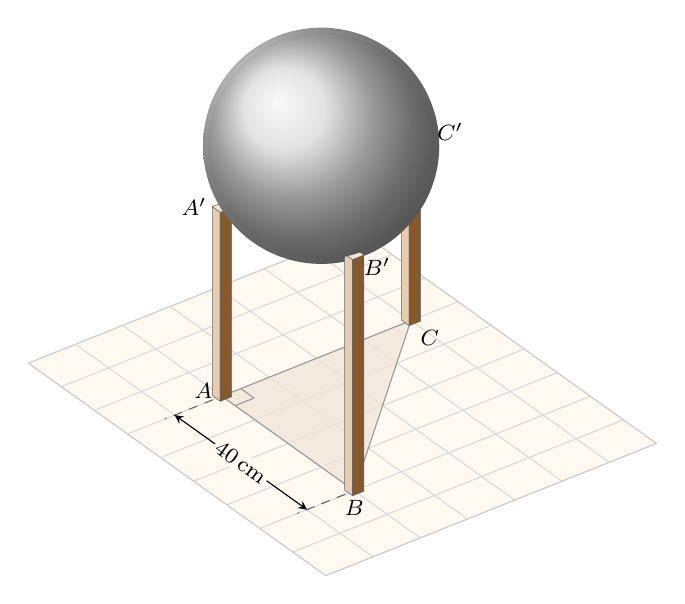
\begin{tikzpicture}[scale=0.6, font=\footnotesize, line join=round, line cap=round, >=stealth, x={(0.7cm, -0.5cm)}, y={(1cm, 0.4cm)}, z={(0cm, 1cm)}]
			\def\SanTrai{-3}      
			\def\SanPhai{6}       
			\def\SanDuoi{-2}      
			\def\SanTren{5}         
			\pgfmathtruncatemacro{\Xnext}{\SanTrai + 1}
			\pgfmathtruncatemacro{\Ynext}{\SanDuoi + 1}
			\fill[orange!5] (\SanTrai,\SanDuoi,0) -- (\SanPhai,\SanDuoi,0) -- (\SanPhai,\SanTren,0) -- (\SanTrai,\SanTren,0) -- cycle;
			\begin{scope}
				\clip (\SanTrai,\SanDuoi,0) -- (\SanPhai,\SanDuoi,0) -- (\SanPhai,\SanTren,0) -- (\SanTrai,\SanTren,0) -- cycle;
				\foreach \x in {\SanTrai, \Xnext, ..., \SanPhai} 
				\draw[gray!30, thin] (\x,\SanDuoi,0) -- (\x,\SanTren,0);
				\foreach \y in {\SanDuoi, \Ynext, ..., \SanTren} 
				\draw[gray!30, thin] (\SanTrai,\y,0) -- (\SanPhai,\y,0);
			\end{scope}
			\draw[gray!40, thin] (\SanTrai,\SanDuoi,0) -- (\SanPhai,\SanDuoi,0) -- (\SanPhai,\SanTren,0) -- (\SanTrai,\SanTren,0) -- cycle;
			\draw[fill=brown!20, fill opacity=0.8, draw=gray!80, thin] (0,0,0) -- (4,0,0) -- (0,4,0) -- cycle;
			\draw[draw=gray!80, thin] (0.4,0,0) -- (0.4,0.4,0) -- (0,0.4,0);
			\draw[dashed, thin, gray!80!black] (0, -0.2, 0) -- (0, -1.2, 0) (4, -0.2, 0) -- (4, -1.2, 0);
			\draw[<->, thin] (0, -1.0, 0) -- (4, -1.0, 0) 
			node[midway, fill=orange!5, inner sep=1pt,sloped] {$40\mathrm{\,cm}$};
			\newcommand{\drawpost}[3]{
				\def\w{0.12} 
				\coordinate (P1) at (#1-\w, #2-\w, 0);
				\coordinate (P2) at (#1+\w, #2-\w, 0);
				\coordinate (P3) at (#1+\w, #2+\w, 0);
				\coordinate (P4) at (#1-\w, #2+\w, 0);
				\coordinate (T1) at (#1-\w, #2-\w, #3);
				\coordinate (T2) at (#1+\w, #2-\w, #3);
				\coordinate (T3) at (#1+\w, #2+\w, #3);
				\coordinate (T4) at (#1-\w, #2+\w, #3);
				\draw[fill=brown!40, draw=black!60, very thin] (P1) -- (P2) -- (T2) -- (T1) -- cycle;
				\draw[fill=brown!70!black, draw=black!60, very thin] (P2) -- (P3) -- (T3) -- (T2) -- cycle;
				\draw[fill=brown!20, draw=black!60, very thin] (T1) -- (T2) -- (T3) -- (T4) -- cycle;
			}
			\drawpost{0}{4}{4} % Cọc C' 
			\drawpost{0}{0}{4} % Cọc A' 
			\shade[ball color=white!70!gray] (-7, 7, -1) circle (2.5cm);
			\drawpost{4}{0}{5} % Cọc B' 		
			\node[left, yshift=2pt] at (0, 0, 0) {$A$};
			\shade[ball color=white!70!gray] (-7, 7, -1) circle (2.4cm);
			\node[below] at (4, 0, 0) {$B$};
			\node[below right] at (0, 4, 0){$C$};
			\node[left, xshift=-2pt] at (0, 0, 4) {$A'$};
			\node[below right, yshift=2pt] at (4, 0, 5) {$B'$};
			\node[right, xshift=6pt] at (0, 4, 4) {$C'$};
		\end{tikzpicture}
	}	
	\par
	\shortans[0]{179}
	\loigiai{
		\begin{center}
			\begin{tikzpicture}[
				>=stealth,line join=round,line cap=round,
				every node/.style={font=\scriptsize},
				declare function={
					xb=2.2; yc=3;
					za=2; zb=2; zc=2.8;
					ux_angle=220;
					sph_x=7.5; sph_y=1.5;
					R=2; ycs=-0.7;
					r=sqrt (R*R - ycs*ycs);
					b=0.45;
					Hy=-4.2;
					plane_w=1.2;
				}
				]
				\path (0,0) coordinate (O);
				\path (ux_angle:1) coordinate (ux);
				\path (0:1) coordinate (uy);
				\path (90:1) coordinate (uz);
				\draw[-stealth,line width=0.7pt,red!70!black] (O) -- ($3.5*(ux)$) node[below] {$x$};
				\draw[-stealth,line width=0.7pt,red!70!black] (O) -- ($4.5*(uy)$) node[below] {$y$};
				\draw[-stealth,line width=0.7pt,red!70!black] (O) -- ($3.5*(uz)$) node[left] {$z$};
				\path (O) coordinate (A);
				\path ($xb*(ux)$) coordinate (B);
				\path ($yc*(uy)$) coordinate (C);
				\path ($za*(uz)$) coordinate (A');
				\path (B) ++($zb*(uz)$) coordinate (B');
				\path (C) ++($zc*(uz)$) coordinate (C');
				\draw[line width=0.6pt] (B) -- (B');
				\draw[line width=0.6pt] (C) -- (C');
				\draw[line width=0.6pt] ($1.5*(ux) - 1.2*(uy)$) -- ($5*(ux) - 1.2*(uy)$) -- ($5*(ux) + 4*(uy)$);
				\foreach \p/\pos/\text in {
					A/-45/O \equiv A,
					B/-90/B,
					C/-90/C,
					A'/180/A',
					B'/180/B',
					C'/0/C'
				}{
					\draw (\p) circle (0.6pt) node[shift={(\pos:8pt)}] {$\text$};
				}
				\begin{scope}[shift={(sph_x,sph_y)}]
					\path (0,0) coordinate (I);
					\path (0,R) coordinate (K);
					\path (0,Hy) coordinate (H);
					\draw[line width=0.6pt] (I) circle (R);
					\draw[dash pattern=on 2pt off 1.5pt,line width=0.6pt,smooth,variable=\t] plot[domain=0:180] ({r*cos (\t)},{ycs + b*sin (\t)});
					\draw[line width=0.6pt,smooth,variable=\t] plot[domain=180:360] ({r*cos (\t)},{ycs + b*sin (\t)});
					\draw[dashed,line width=0.6pt] (K) -- (H);
					\draw[line width=0.6pt] (-plane_w,Hy) -- (plane_w,Hy);
					\path (I) -- (K) node[midway,left] {$R$};
					\node[left=2pt] at (-R,0) {$(S)$};
					\foreach \p/\pos/\text in {
						I/0/I,
						K/90/K,
						H/30/H
					}{
						\draw (\p) circle (0.6pt) node[shift={(\pos:8pt)}] {$\text$};
					}
				\end{scope}
			\end{tikzpicture}
		\end{center}
		Gắn hệ trục tọa độ $Oxyz$ với gốc tọa độ $O \equiv A$, trục $Ox$ hướng theo tia $AB$, trục $Oy$ hướng theo tia $AC$, trục $Oz$ hướng theo tia $AA'$ (như hình vẽ).\\
		Đơn vị dài trên mỗi trục là centimet (cm).\\
		Vì tam giác $ABC$ vuông cân tại $A$ và $AB=40$ nên $A(0;0;0)$, $B(40;0;0)$ và $C(0;40;0)$.\\
		Dựa vào độ cao của các cọc, ta có tọa độ các đỉnh cọc là $A'(0;0;60)$, $B'(40;0;70)$, $C'(0;40;80)$.\\
		Rõ ràng mặt cầu giới hạn vật nặng là một mặt cầu $(S)$ có tâm $I(a; b; c)$ và bán kính $R = 60$.\\
		Do ba đỉnh cọc $A'$, $B'$, $C'$ đều chạm vào mặt cầu nên khoảng cách từ $I$ đến các đỉnh cọc đều bằng $R$.\\ 
		Ta có hệ phương trình
		\begin{align}
			& A'I^2 = a^2 + b^2 + (c-60)^2 = 60^2 \quad &(1) \notag \\
			& B'I^2 = (a-40)^2 + b^2 + (c-70)^2 = 60^2 \quad &(2) \notag \\
			& C'I^2 = a^2 + (b-40)^2 + (c-80)^2 = 60^2 \quad &(3) \notag
		\end{align}
		Lấy phương trình $(2)$ trừ đi phương trình $(1)$ vế theo vế, ta được
		\[ -80a + 1\,600 - 20c + 1\,300 = 0 \Leftrightarrow 20c = -80a + 2\,900 \Leftrightarrow c = -4a + 145. \]
		Lấy phương trình $(3)$ trừ đi phương trình $(1)$ vế theo vế, ta được
		\[ -80b + 1\,600 - 40c + 2\,800 = 0 \Leftrightarrow 80b = -40c + 4\,400 \Leftrightarrow b = -\dfrac{1}{2}c + 55. \]
		Thế $c = -4a + 145$ vào biểu thức của $b$, ta có
		\[ b = -\dfrac{1}{2}(-4a + 145) + 55 = 2a - \dfrac{145}{2} + 55 = 2a - \dfrac{35}{2}. \]
		Thế $b$ và $c$ vào phương trình $(1)$, ta thu được
		\allowdisplaybreaks
		\begin{align*}
			& a^2 + \left(2a - \dfrac{35}{2}\right)^2 + (-4a + 145 - 60)^2 = 60^2 \\
			\Leftrightarrow \;& a^2 + 4a^2 - 70a + \dfrac{1\,225}{4} + (-4a + 85)^2 = 3\,600 \\
			\Leftrightarrow \;& 5a^2 - 70a + 306{,}25 + 16a^2 - 680a + 7\,225 = 3\,600 \\
			\Leftrightarrow \;& 21a^2 - 750a + 3\,931{,}25 = 0 \\
			\Leftrightarrow \;& 84a^2 - 3\,000a + 15\,725 = 0.
		\end{align*}
		Giải phương trình bậc hai trên, ta nhận được hai nghiệm $a$
		\[
		\hoac{
			& a = \dfrac{750 + 5\sqrt{9\,291}}{42} \Rightarrow c = -4\left(\dfrac{750 + 5\sqrt{9\,291}}{42}\right) + 145 = \dfrac{1\,545 - 10\sqrt{9\,291}}{21} \\
			& a = \dfrac{750 - 5\sqrt{9\,291}}{42} \Rightarrow c = -4\left(\dfrac{750 - 5\sqrt{9\,291}}{42}\right) + 145 = \dfrac{1\,545 + 10\sqrt{9\,291}}{21}.
		}
		\]
		Theo tính thực tế, ta đặt vật nặng từ trên xuống cho nên mặt cầu sẽ nằm phía trên các đỉnh cọc. Tức là ta phải lấy giá trị độ cao của tâm quả cầu $c$ lớn hơn.\\
		So sánh hai giá trị $\dfrac{1\,545 - 10\sqrt{9\,291}}{21}$ và $\dfrac{1\,545 + 10\sqrt{9\,291}}{21}$.\\
		Ta chọn $c = \dfrac{1\,545 + 10\sqrt{9\,291}}{21}$.\\
		Gọi $K$ là điểm cao nhất của mặt cầu và $H$ là hình chiếu của $I$ xuống mặt đất (như hình vẽ bên phải).\\ Khi đó, độ cao của quả cầu so với mặt đất chính là đoạn $KH$.\\
		Ta có
		\[ KH = KI + IH = R + c = 60 + \dfrac{1\,545 + 10\sqrt{9\,291}}{21} = \dfrac{2\,805 + 10\sqrt{9\,291}}{21} \approx 179\,\,\mathrm{\,(cm)}. \]
		Vậy độ cao của vật nặng so với mặt đất xấp xỉ $179$\,cm.
	}
\end{ex}
%%%=============================%%%

%%%=============EX_19=============%%%
\begin{ex}%[1D3V3-5]%[TDMT13]%[Nguyễn Đăng Ái]
	Câu chuyện về mối tình đầu của giới trẻ thì nó rất là thú vị và hấp dẫn, yêu thì nồng nhiệt hết mình mà chia tay thì cũng phũ phàng quyết liệt không kém. Thế nhưng dù có như thế nào thì mối tình đầu cũng rất là khó phai.\\
	Giả sử có một mối tình đầu giữa hai bạn \textbf{Bình} và \textbf{An} khi còn yêu nhau ta coi như có $100$ điểm tình cảm. Vào một ngày nọ, vì một số lí do hiểu lầm không thể nào giải thích giữa đôi nam nữ này mà dẫn tới họ quyết định chia tay nhau. Ở những ngày sau đó coi như họ gặp nhau mỗi ngày một lần, coi như sau một ngày không gặp nhau thì điểm tình cảm giảm đi $30\%$ so với lúc vừa gặp nhau xong, ngay sau mỗi lần gặp nhau điểm tình cảm lại tăng thêm $12$ điểm so với ngay trước đó. Với giả sử điểm tình cảm nhỏ hơn $30$ thì coi như quên hẳn được nhau và khi gặp sẽ không còn tăng thêm được điểm tình cảm nữa. Hỏi sau tối thiểu bao nhiêu ngày kể từ lúc chia tay thì hai bạn này quên được nhau (\textit{làm tròn kết quả đến hàng đơn vị})?
	\par
	\shortans[0]{10}
	\loigiai{
		Gọi $u_n$ là điểm tình cảm của hai bạn Bình và An sau $n$ ngày tính từ lúc chia tay và ngay trước khi gặp nhau ở lần tiếp theo ($n \in \mathbb{N}^*$).\\
		Ban đầu, điểm tình cảm là $u_0 = 100$.\\
		Sau $1$ ngày đầu tiên (ngay trước khi gặp lần $1$), điểm tình cảm giảm $30\%$
		\[ u_1 = u_0 - 0{,}3u_0 = 0{,}7u_0. \]
		Ngay sau khi gặp nhau lần $1$, điểm tình cảm là $u_1 + 12$.\\
		Sau $2$ ngày (ngay trước khi gặp lần $2$), điểm tình cảm lại giảm $30\%$ so với lúc vừa gặp
		\[ u_2 = 0{,}7(u_1 + 12) = 0{,}7 \cdot u_1 + 12 \cdot 0{,}7 = 0{,}7^2u_0 + 12 \cdot 0{,}7. \]
		Ngay sau khi gặp nhau lần $2$, điểm tình cảm là $u_2 + 12$.\\
		Sau $3$ ngày (ngay trước khi gặp lần $3$)
		\[ u_3 = 0{,}7(u_2 + 12) = 0{,}7\left(0{,}7^2u_0 + 12 \cdot 0{,}7\right) + 12 \cdot 0{,}7 = 0{,}7^3u_0 + 12 \cdot 0{,}7^2 + 12 \cdot 0{,}7. \]
		Bằng phương pháp quy nạp, ta suy ra điểm tình cảm ngay trước lần gặp thứ $n$ là
		\[ u_n = 0{,}7^n u_0 + 12 \left( 0{,}7 + 0{,}7^2 + \dots + 0{,}7^{n-1} \right). \]
		Biểu thức trong ngoặc là tổng của $n-1$ số hạng đầu tiên của một cấp số nhân có số hạng đầu $u_1' = 0{,}7$ và công bội $q = 0{,}7$. Áp dụng công thức tính tổng cấp số nhân, ta được
		\[ 0{,}7 + 0{,}7^2 + \dots + 0{,}7^{n-1} = 0{,}7 \cdot \dfrac{1 - 0{,}7^{n-1}}{1 - 0{,}7} = \dfrac{0{,}7 - 0{,}7^n}{0{,}3}. \]
		Do đó, công thức tổng quát của dãy số là
		\allowdisplaybreaks
		\begin{align*}
			u_n &= 0{,}7^n \cdot 100 + 12 \cdot \dfrac{0{,}7 - 0{,}7^n}{0{,}3} \\
			&= 100 \cdot 0{,}7^n + 40\left(0{,}7 - 0{,}7^n\right) \\
			&= 60 \cdot 0{,}7^n + 28.
		\end{align*}
		Theo giả thiết, hai bạn sẽ quên hẳn nhau khi điểm tình cảm nhỏ hơn $30$ ngay trước khi gặp lần tiếp theo.\\ 
		Ta có bất phương trình
		\allowdisplaybreaks
		\begin{align*}
			& u_n < 30 \\
			\Leftrightarrow \;& 60 \cdot 0{,}7^n + 28 < 30 \\
			\Leftrightarrow \;& 60 \cdot 0{,}7^n < 2 \\
			\Leftrightarrow \;& 0{,}7^n < \dfrac{1}{30} \\
			\Leftrightarrow \;& n > \log_{0{,}7} \left( \dfrac{1}{30} \right) \approx 9{,}53 \dots
		\end{align*}
		Vì $n$ là số ngày nên $n$ phải là số nguyên dương, suy ra giá trị tối thiểu của $n$ là $10$.\\
		Vậy sau tối thiểu $10$ ngày kể từ lúc chia tay thì hai bạn sẽ quên được nhau.
	}
\end{ex}
%%%=============================%%%

%%%=============EX_20=============%%%
\begin{ex}%[2D6C1-4]%[TDMT13]%[Hà Văn Hảo]
	Trong $15$ bóng bida, tiến hành bốc ngẫu nhiên $3$ bóng chia cho cơ thủ $X$, sau đó lại bốc $3$ bóng chia cho cơ thủ $Y$. Gọi $A$ là biến cố có ít nhất một trong hai cơ thủ được ba bóng là ba số tự nhiên liên tiếp, $B$ là biến cố cả hai cơ thủ được ba bóng là ba số tự nhiên liên tiếp. Hãy tính $\mathrm{P}(A) + \mathrm{P}(B\mid A)$ (\textit{làm tròn kết quả đến hàng phần trăm}).
	\par
	\shortans[0]{0{,}08}
	\loigiai{
		Phép thử: Bốc ngẫu nhiên $3$ bóng cho cơ thủ $X$, sau đó bốc tiếp $3$ bóng cho cơ thủ $Y$.\\
		Số phần tử của không gian mẫu là $n(\Omega) = \mathrm{C}_{15}^3 \cdot \mathrm{C}_{12}^3 = 100\,100$.\\
		Gọi $E$ là biến cố: \lq\lq Cơ thủ $X$ được $3$ bóng là ba số tự nhiên liên tiếp\rq\rq.\\
		Gọi $F$ là biến cố: \lq\lq Cơ thủ $Y$ được $3$ bóng là ba số tự nhiên liên tiếp\rq\rq.\\
		Khi đó, biến cố $A = E \cup F$ và biến cố $B = E \cap F$.\\
		Trong $15$ bóng, có $13$ bộ ba số tự nhiên liên tiếp là $\{1;2;3\}$, $\{2;3;4\}$, $\ldots$, $\{13;14;15\}$.
		\begin{itemize}
			\item Số kết quả thuận lợi cho $E$ là chọn $1$ bộ cho $X$ và $3$ bóng bất kì từ $12$ bóng còn lại cho $Y$.\\ Suy ra $n(E) = \mathrm{C}_{13}^1 \cdot \mathrm{C}_{12}^3 = 2\,860$.
			\item Hoàn toàn tương tự, vai trò của $Y$ như $X$ nên $n(F) = \mathrm{C}_{13}^1 \cdot \mathrm{C}_{12}^3 = 2\,860$.
			\item Để tính $n(E \cap F)$ (cả hai cùng được ba số liên tiếp), ta phân tích các lựa chọn của $X$ ảnh hưởng đến $Y$ như sau
			\begin{itemize}
				\item Nếu $X$ lấy bộ $\{1;2;3\}$, $Y$ có thể lấy từ bộ $\{4;5;6\}$ đến $\{13;14;15\}$ $\Rightarrow$ có $10$ cách.
				\item Nếu $X$ lấy bộ $\{2;3;4\}$, $Y$ có thể lấy từ bộ $\{5;6;7\}$ đến $\{13;14;15\}$ $\Rightarrow$ có $9$ cách.
				\item Nếu $X$ lấy một trong $9$ bộ ở giữa (từ $\{3;4;5\}$ đến $\{11;12;13\}$), mỗi bộ của $X$ sẽ làm mất đi $5$ bộ liên tiếp có thể chọn của $Y$.\\ Vậy $Y$ còn $13 - 5 = 8$ cách $\Rightarrow$ có $9 \cdot 8 = 72$ cách.
				\item Nếu $X$ lấy bộ $\{12;13;14\}$, $Y$ có thể lấy từ bộ $\{1;2;3\}$ đến $\{9;10;11\}$ $\Rightarrow$ có $9$ cách.
				\item Nếu $X$ lấy bộ $\{13;14;15\}$, $Y$ có thể lấy từ bộ $\{1;2;3\}$ đến $\{10;11;12\}$ $\Rightarrow$ có $10$ cách.
			\end{itemize}
			Suy ra $n(B) = n(E \cap F) = 10 + 9 + 72 + 9 + 10 = 110$.
		\end{itemize}
		Theo quy tắc cộng mở rộng cho tập hợp, ta có
		\[ n(A) = n(E \cup F) = n(E) + n(F) - n(E \cap F) = 2\,860 + 2\,860 - 110 = 5\,610. \]
		Theo định nghĩa xác suất có điều kiện $\mathrm{P}(B \mid A) = \dfrac{\mathrm{P}(B \cap A)}{\mathrm{P}(A)}$.\\
		Vì $B \subset A$ nên $B \cap A = B$, do đó $\mathrm{P}(B \mid A) = \dfrac{\mathrm{P}(B)}{\mathrm{P}(A)} = \dfrac{n(B)}{n(A)}$.\\
		Vậy giá trị biểu thức cần tính là
		\allowdisplaybreaks
		\begin{align*}
			\mathrm{P}(A) + \mathrm{P}(B\mid A) = \dfrac{n(A)}{n(\Omega)} + \dfrac{n(B)}{n(A)} 
			= \dfrac{5\,610}{\mathrm{C}_{15}^3 \cdot \mathrm{C}_{12}^3} + \dfrac{110}{5\,610}
			= \dfrac{5\,610}{100\,100} + \dfrac{110}{5\,610} \approx 0{,}08.
		\end{align*}
	}
\end{ex}
%%%=============================%%%

%%%==============EX_21==============%%%
\begin{ex}%[2D4V3-4]%[TDMT13]%[Lê Hồ Quang Minh]
	\immini[thm]{Cho hình phẳng $(H)$ giới hạn bởi hai phần parabol giống nhau, một phần có trục đối xứng thẳng đứng và một phần có trục đối xứng tạo với phương thẳng đứng một góc $60^\circ$. Các kích thước được cho như hình vẽ bên dưới. Hãy tính diện tích của hình phẳng $(H)$ theo đơn vị centimét vuông \textit{(làm tròn kết quả đến hàng đơn vị).}}
	{\begin{tikzpicture}[scale=.5,>=stealth,line join=round,line cap=round,x=0.15cm,y=0.15cm,every node/.style={font=\scriptsize}]
			\tikzset{
				declare function={
					a = 7/32;
					xB = -8;
					yB = 14;
					xA = 32*sqrt (3)/7 + 8;
					yA = a*xA*xA;
					f (\x) = a*\x*\x;
					ang = 60;
					yI = 8*sqrt (3) + 14;
				}
			}
			\draw[dashed,line width=0.6pt] (-17,14) -- (-8,14);
			\draw[dashed,line width=0.6pt] (-17,0) -- (16,0);
			\draw[dashed,line width=0.6pt] (-8,14) -- (-8,-3);
			\draw[dashed,line width=0.6pt] (0,0) -- (0,-3);
			\draw[stealth-stealth,line width=0.6pt] (-15,0) -- (-15,14) node[midway,left] {$14$\,cm};
			\draw[stealth-stealth,line width=0.6pt] (-8,-2) -- (0,-2) node[midway,below] {$8$\,cm};
			\draw[dashed,line width=0.6pt] (0,-3) -- (0,42);
			\begin{scope}[shift={(xB,yB)},rotate=ang,yscale=-1,rotate=-ang,shift={(-xB,-yB)}]
				\draw[dashed,line width=0.6pt] (0,0) -- (0,42);
			\end{scope}
			\draw[line width=0.6pt] (0,yI) ++(90:4) arc (90:30:4);
			\node at ($(0,yI) + (60:6.5)$) {$60^\circ$};
			\fill (0,yI) circle (1pt);
			\fill (-8,14) circle (1pt);
			\fill (0,0) circle (1pt);
			\fill (xA,yA) circle (1pt);
			\draw[line width=1pt,draw=red!70!black] plot[smooth,samples=200,domain=xB:xA] (\x,{f (\x)});
			\begin{scope}[shift={(xB,yB)},rotate=ang,yscale=-1,rotate=-ang,shift={(-xB,-yB)}]
				\draw[line width=1pt,draw=red!70!black] plot[smooth,samples=200,domain=xB:xA] (\x,{f (\x)});
			\end{scope}
	\end{tikzpicture}}
	\par 
	\shortans[0]{998}
	\loigiai{
		\immini{Dễ dàng nhận ra sự đối xứng của hình phẳng $(H)$, do đó đường thẳng đi qua hai điểm $A$ và $B$ sẽ chia $(H)$ thành hai phần có diện tích bằng nhau.\\
		Gắn hệ trục tọa độ $Oxy$ sao cho gốc $O$ trùng với đỉnh của parabol bên dưới và trục $Oy$ trùng với trục đối xứng của nó (như hình vẽ).\\
		Dựa vào các kích thước đã cho, ta xác định được tọa độ điểm $B$ là $B(-8; 14)$.\\
		Gọi $(P)$ là phần parabol có đỉnh $O$.\\ Phương trình của $(P)$ có dạng $y = ax^2$ ($a > 0$).\\
		Vì $(P)$ đi qua $B(-8; 14)$ nên ta có
		\[ 14 = a \cdot (-8)^2 \Rightarrow a = \dfrac{14}{64} = \dfrac{7}{32}. \]
		Suy ra phương trình parabol là $(P) \colon y = \dfrac{7}{32}x^2$.}{
		\begin{tikzpicture}[scale=1,>=stealth,line join=round,line cap=round,x=0.15cm,y=0.15cm,every node/.style={font=\scriptsize}]
			\tikzset{
				declare function={
					a = 7/32;
					xB = -8;
					yB = 14;
					xA = 32*sqrt (3)/7 + 8;
					yA = a*xA*xA;
					f (\x) = a*\x*\x;
					ang = 60;
					yI = 8*sqrt (3) + 14;
				}
			}
			\draw[-stealth,line width=0.7pt] (-22,0) -- (22,0) node[below] {$x$};
			\draw[-stealth,line width=0.7pt] (0,-4) -- (0,62) node[shift={(-6pt,-5pt)}] {$y$};
			\draw[dashed,line width=0.6pt] (-17,14) -- (-8,14);
			\draw[dashed,line width=0.6pt] (-8,14) -- (-8,-3);
			\draw[dashed,line width=0.6pt] (0,0) -- (0,-3);
			\draw[stealth-stealth,line width=0.6pt] (-15,0) -- (-15,14) node[midway,left] {$14$\,cm};
			\draw[stealth-stealth,line width=0.6pt] (-8,-2) -- (0,-2) node[midway,below] {$8$\,cm};
			\draw[dashed,line width=0.6pt] (-16,{sqrt (3)*(-16+8)+14}) -- (18,{sqrt (3)*(18+8)+14});
			\begin{scope}[shift={(xB,yB)},rotate=ang,yscale=-1,rotate=-ang,shift={(-xB,-yB)}]
				\draw[dashed,line width=0.6pt] (0,0) -- (0,42);
			\end{scope}
			\draw[line width=0.6pt] (0,yI) ++(240:4) arc (240:270:4);
			\node at ($(0,yI) + (255:6.5)$) {$30^\circ$};
			\draw[line width=0.6pt] (0,yI) ++(210:4) arc (210:240:4);
			\node at ($(0,yI) + (225:6.5)$) {$30^\circ$};
			\draw[line width=0.6pt] (-8,14) ++(180:3.5) arc (180:240:3.5);
			\node at ($(-8,14) + (210:5)$) {$60^\circ$};
			\fill (0,yI) circle (1pt);
			\fill (-8,14) circle (1pt) node[above left] {$B$};
			\fill (0,0) circle (1pt) node[below right] {$O$};
			\fill (xA,yA) circle (1pt) node[right] {$A$};
			\begin{scope}
				%\clip (-22,-4) rectangle (22,62);
				\draw[line width=1pt,draw=red!70!black] plot[smooth,samples=200,domain=xB:xA] (\x,{f (\x)});
				\begin{scope}[shift={(xB,yB)},rotate=ang,yscale=-1,rotate=-ang,shift={(-xB,-yB)}]
					\draw[line width=1pt,draw=red!70!black] plot[smooth,samples=200,domain=xB:xA] (\x,{f (\x)});
				\end{scope}
			\end{scope}
		\end{tikzpicture}}
		Đường thẳng $AB$ đi qua điểm $B(-8;14)$ và tạo với chiều dương trục $Ox$ một góc $60^\circ$, nên có hệ số góc $k = \tan 60^\circ = \sqrt{3}$.\\
		Phương trình đường thẳng $AB$ là
		\[ y = \sqrt{3}\left[x - (-8)\right] + 14 \Leftrightarrow y = \sqrt{3}x + 8\sqrt{3} + 14. \]
		Xét phương trình hoành độ giao điểm của đường thẳng $AB$ và parabol $(P)$
		\[ \dfrac{7}{32}x^2 = \sqrt{3}x + 8\sqrt{3} + 14 \Leftrightarrow \dfrac{7}{32}x^2 - \sqrt{3}x - 8\sqrt{3} - 14 = 0. \]
		Giải phương trình trên, ta thu được hai nghiệm
		\[ \hoac{&x = -8=x_B \\ &x = \dfrac{56 + 32\sqrt{3}}{7}=x_A.} \]
		Do tính đối xứng, diện tích hình phẳng $(H)$ bằng $2$ lần diện tích hình phẳng giới hạn bởi đường thẳng $AB$ và parabol $(P)$.\\ 
		Ta có
		\[
			S_{(H)} = 2 \displaystyle\int\limits_{-8}^{\frac{56 + 32\sqrt{3}}{7}} \left[ \left( \sqrt{3}x + 8\sqrt{3} + 14 \right) - \dfrac{7}{32}x^2 \right] \mathrm{\,d}x 
			\approx 998 \mathrm{\,(cm}^2).
		\]
		Vậy diện tích của hình phẳng $(H)$ xấp xỉ $998$\,cm$^2$.
	}
\end{ex}
%%%=============================%%%

%%%=============EX_22=============%%%
\begin{ex}%[0D8C2-7]%[TDMT13]%[Nguyễn Thành Hậu]
	\immini[thm]{Cho tập $X$ gồm các số nguyên trong đoạn $[1;15]$ và $9$ ô tròn $a$, $b$, $c$, $d$, $e$, $f$, $g$, $h$, $k$ được bố trí như hình vẽ. Mỗi ô tròn nhỏ chỉ xếp được đúng một số. Biết rằng có tất cả $T$ cách chọn ra $9$ số khác nhau từ tập $X$ để xếp vào $9$ ô tròn, sao cho có ít nhất một hàng được sắp xếp theo chiều tăng dần hoặc giảm dần. Hãy xác định bốn chữ số tận cùng của $T$.}{
		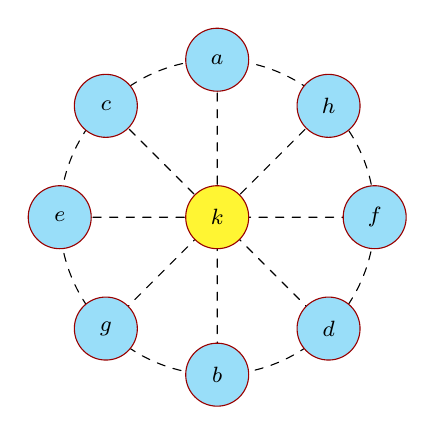
\begin{tikzpicture}[declare function={r=0.4;},line cap=round,line join=round,>=stealth,font=\footnotesize,scale=1]
			\draw[dashed] (0,0) circle (2);
			\path
			(0,0) coordinate (k)
			(0:2) coordinate (f)
			(45:2) coordinate (h)
			(90:2) coordinate (a)
			(135:2) coordinate (c)
			(180:2) coordinate (e)
			(-45:2) coordinate (d)
			(-90:2) coordinate (b)
			(-135:2) coordinate (g);
			\draw[dashed] (e)--(f)
			(c)--(d)
			(a)--(b)
			(h)--(g);
			\foreach \i in {d,f,a,c,e,b,g,h}{
				\filldraw[fill=cyan!40,draw=red!60!black] (\i) circle (r) node[text=black] {$\i$};
			}
			\filldraw[fill=yellow!80,draw=red!60!black] (k) circle (r) node[text=black] {$k$};
		\end{tikzpicture}
	}
	\par
	\shortans[oly]{6320}
	\loigiai{
		Số cách chọn ra $9$ số từ tập $X$ (gồm $15$ phần tử) là $\mathrm{C}_{15}^{9}$ cách.\\
		Mỗi cách chọn ra $9$ số, ta xếp vào $9$ vị trí phân biệt đã được đặt tên, có $9!$ cách.\\
		Do đó, không gian mẫu (tổng số cách xếp ngẫu nhiên) là $n(\Omega) = \mathrm{C}_{15}^{9} \cdot 9! = \mathrm{A}_{15}^{9}$.\\
		Ta sẽ đếm số cách xếp vi phạm yêu cầu bài toán, tức là \textbf{không có hàng nào} được sắp xếp theo chiều tăng dần hoặc giảm dần.\\
		Các hàng thẳng hàng qua tâm $k$ là các bộ ba $(a,k,b)$, $(c,k,d)$, $(e,k,f)$, $(g,k,h)$.\\
		Để một hàng $(x,k,y)$ không tăng dần cũng không giảm dần, thì phần tử ở giữa $k$ không được nằm giữa $x$ và $y$ về mặt giá trị.\\ Nghĩa là $x$ và $y$ phải cùng lớn hơn $k$, hoặc cùng nhỏ hơn $k$.\\
		Nói cách khác, cả $4$ cặp $(a,b)$, $(c,d)$, $(e,f)$, $(g,h)$ đều phải có $2$ phần tử nằm \textbf{cùng phía} so với giá trị của $k$.\\
		Giả sử $9$ số được chọn ra được sắp xếp tăng dần $x_1 < x_2 < x_3 < x_4 < x_5 < x_6 < x_7 < x_8 < x_9$.\\
		Vì các phần tử ở $8$ ô bên ngoài luôn đi theo từng cặp nằm cùng phía so với $k$, nên số lượng phần tử lớn hơn $k$ và nhỏ hơn $k$ đều phải là số chẵn.\\ Do đó, $k$ chỉ có thể nhận các giá trị ở vị trí lẻ $k \in \{x_1, x_3, x_5, x_7, x_9\}$.\\
		Ta biểu diễn số cách xếp vi phạm tương ứng với mỗi lựa chọn của $k$ qua sơ đồ sau
		\begin{center}
			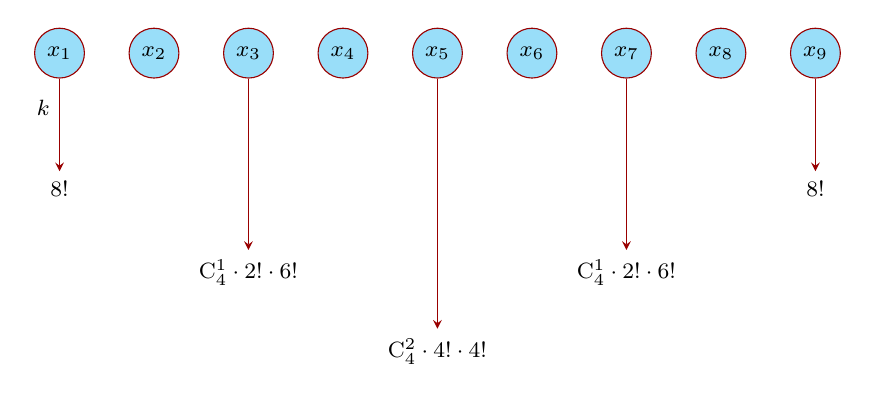
\begin{tikzpicture}[>=stealth,font=\footnotesize,scale=1]
				\foreach \i in {1,2,3,4,5,6,7,8,9}{
					\node[draw=red!60!black,fill=cyan!40,circle,inner sep=1pt,minimum size=18pt] (x\i) at (\i*1.2,0) {$x_{\i}$};
				}
				\draw[->,color=red!60!black] (x1) -- ++(0,-1.5) node[below,text=black] {$8!$};
				\node at (1.2,-0.7) [left] {$k$};
				\draw[->,color=red!60!black] (x3) -- ++(0,-2.5) node[below,text=black] {$\mathrm{C}_4^1 \cdot 2! \cdot 6!$};
				\draw[->,color=red!60!black] (x5) -- ++(0,-3.5) node[below,text=black] {$\mathrm{C}_4^2 \cdot 4! \cdot 4!$};
				\draw[->,color=red!60!black] (x7) -- ++(0,-2.5) node[below,text=black] {$\mathrm{C}_4^1 \cdot 2! \cdot 6!$};
				\draw[->,color=red!60!black] (x9) -- ++(0,-1.5) node[below,text=black] {$8!$};
			\end{tikzpicture}
		\end{center}
		\textit{Giải thích sơ đồ:}
		\begin{itemize}
			\item Nếu $k = x_1$ (hoặc $x_9$): $8$ phần tử còn lại đều lớn hơn (hoặc nhỏ hơn) $k$, ta xếp tùy ý vào $8$ vị trí xung quanh có $8!$ cách.
			\item Nếu $k = x_3$ (hoặc $x_7$): Có $2$ phần tử nhỏ hơn $k$ và $6$ phần tử lớn hơn $k$. Ta phải chọn $1$ đường chéo trong $4$ đường chéo để đặt $2$ phần tử nhỏ hơn này ($\mathrm{C}_4^1$ cách), hoán vị $2$ phần tử đó ($2!$ cách), và xếp $6$ phần tử còn lại vào $6$ ô trống ($6!$ cách).
			\item Nếu $k = x_5$: có $4$ phần tử nhỏ hơn $k$ và $4$ phần tử lớn hơn $k$. Ta chọn $2$ đường chéo cho $4$ phần tử nhỏ hơn ($\mathrm{C}_4^2$ cách), hoán vị chúng ($4!$ cách), xếp $4$ phần tử lớn hơn vào $4$ ô còn lại ($4!$ cách).
		\end{itemize}
		Tổng số cách xếp vi phạm đối với một bộ $9$ số được chọn là
		\[S_{vp} = 2 \cdot 8! + 2 \cdot \left(\mathrm{C}_4^1 \cdot 2! \cdot 6!\right) + \mathrm{C}_4^2 \cdot 4! \cdot 4! = 95\,616. \]
		Tổng số cách xếp thỏa mãn (ít nhất một hàng tăng hoặc giảm dần) là
		\begin{align*}
			T &= \mathrm{C}_{15}^{9} \cdot 9! - \mathrm{C}_{15}^{9} \cdot S_{vp} \\
			&= \mathrm{C}_{15}^{9} \cdot \left[9! - \left(2 \cdot 8! + 2 \cdot \mathrm{C}_4^1 2! 6! + \mathrm{C}_4^2 4! 4! \right) \right] \\
			&= 5005 \cdot (362\,880 - 95\,616) = 1\,337\,656\,320.
		\end{align*}
		Vậy bốn chữ số tận cùng của $T$ là $6\,320$.
	}
\end{ex}
%%%=============================%%%
\Closesolutionfile{ans}
\newpage
\indapan{12}{ans/ansTN-Dung}
\indapan[TF]{2}{ans/ansTN-DungSai}
\indapan[SA]{6}{ans/ansTN-DienKhuyet}
%%%%%%%%%%%%%%
%%nhãn kết thúc đề (để đếm số trang tự động mỗi đề)
\label{B\thedeso}